\documentclass[openany]{book}

\usepackage[margin=1in]{geometry}
\usepackage{amsmath,amsfonts,amsthm}
\usepackage{xcolor}
\renewcommand{\familydefault}{ppl}
\newcommand{\E}{\mathbb{E}}
\newcommand{\F}{\mathbb{F}}
\newcommand{\R}{\mathbb{R}}
\newcommand{\la}{\langle}
\newcommand{\ra}{\rangle}
\newcommand{\colim}{\text{colim}}
\newcommand{\T}{\mathcal{T}}
\DeclareMathOperator{\im}{im}
% command+/

\usepackage{quiver}
\usepackage{tikz-cd}


\usepackage{thmtools,thm-restate}

% Fixing mdframed skip below
% See https://tex.stackexchange.com/a/292090/143086
\usepackage[framemethod=TikZ]{mdframed}
\usepackage{xpatch}
\makeatletter
\xpatchcmd{\endmdframed}
	{\aftergroup\endmdf@trivlist\color@endgroup}
	{\endmdf@trivlist\color@endgroup\@doendpe}
	{}{}
\makeatother

\definecolor{huilightpink}{HTML}{fcf2f9}
\definecolor{huidarkpink}{HTML}{ed34b3}
\declaretheoremstyle[
	mdframed={
		backgroundcolor=huilightpink,
		linecolor=huidarkpink,
		rightline=false,
		topline=false,
		bottomline=false,
		linewidth=2pt,
		innertopmargin=5pt,
		innerbottommargin=8pt,
		innerleftmargin=8pt,
		leftmargin=-2pt,
		skipbelow=2pt,
		nobreak
	},
	headfont=\normalfont\bfseries\color{huidarkpink}
]{huipinkbox}
\declaretheorem[style=huipinkbox,name=Theorem,within=chapter]{thm}
\declaretheorem[style=huipinkbox,name=Theorem,sibling=thm]{theorem}



\definecolor{huilightpurple}{HTML}{faf2ff}
\definecolor{huidarkpurple}{HTML}{912ed9}
\declaretheoremstyle[
	mdframed={
		backgroundcolor=huilightpurple,
		linecolor=huidarkpurple,
		rightline=false,
		topline=false,
		bottomline=false,
		linewidth=2pt,
		innertopmargin=5pt,
		innerbottommargin=8pt,
		innerleftmargin=8pt,
		leftmargin=-2pt,
		skipbelow=2pt,
		nobreak
	},
	headfont=\normalfont\bfseries\color{huidarkpurple}
]{huipurplebox}
\declaretheorem[style=huipurplebox,name=Proposition,within=chapter]{prop}

\definecolor{huilightpurple}{HTML}{faf2ff}
\definecolor{huidarkpurple}{HTML}{912ed9}
\declaretheoremstyle[
	mdframed={
		backgroundcolor=huilightpurple,
		linecolor=huidarkpurple,
		rightline=false,
		topline=false,
		bottomline=false,
		linewidth=2pt,
		innertopmargin=5pt,
		innerbottommargin=8pt,
		innerleftmargin=8pt,
		leftmargin=-2pt,
		skipbelow=2pt,
		nobreak
	},
	headfont=\normalfont\bfseries\color{huidarkpurple}
]{huipurplebox}
\declaretheorem[style=huipurplebox,name=Lemma,within=chapter]{lem}

\declaretheorem[style=huipurplebox,name=Corollary,within=chapter]{cor}


\definecolor{huilightblue}{HTML}{edf9ff}
\definecolor{huidarkblue}{HTML}{4b79db}
\declaretheoremstyle[
	mdframed={
		backgroundcolor=huilightblue,
		linecolor=huidarkblue,
		rightline=false,
		topline=false,
		bottomline=false,
		linewidth=2pt,
		innertopmargin=5pt,
		innerbottommargin=8pt,
		innerleftmargin=8pt,
		leftmargin=-2pt,
		skipbelow=2pt,
		nobreak
	},
	headfont=\normalfont\bfseries\color{huidarkblue}
]{huiblueblox}
\declaretheorem[style=huiblueblox,name=Definition,within=chapter]{defn}

\definecolor{huilightblue}{HTML}{edf9ff}
\definecolor{huidarkblue}{HTML}{4b79db}
\declaretheoremstyle[
	mdframed={
		backgroundcolor=huilightblue,
		linecolor=huidarkblue,
		rightline=false,
		topline=false,
		bottomline=false,
		linewidth=2pt,
		innertopmargin=5pt,
		innerbottommargin=8pt,
		innerleftmargin=8pt,
		leftmargin=-2pt,
		skipbelow=2pt,
		nobreak
	},
	headfont=\normalfont\bfseries\color{huidarkblue}
]{huiblueblox}
\declaretheorem[style=huiblueblox,name=Example,within=chapter]{example}

\declaretheoremstyle[
	mdframed={
		backgroundcolor=huilightblue,
		linecolor=huidarkblue,
		rightline=false,
		topline=false,
		bottomline=false,
		linewidth=2pt,
		innertopmargin=5pt,
		innerbottommargin=8pt,
		innerleftmargin=8pt,
		leftmargin=-2pt,
		skipbelow=2pt,
		nobreak
	},
	headfont=\normalfont\bfseries\color{huidarkblue}
]{huiblueblox}
\declaretheorem[style=huiblueblox,name=Problem,within=chapter]{prob}

\newcommand{\nirwarnsymbol}{%
	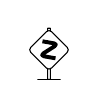
\begin{tikzpicture}[baseline=(x.base)]
		\draw[rounded corners=.01em] (-.05em,-1.07em)rectangle(.05em,.78em);
		\draw[fill=white,rounded corners=1.3] (0,.75em)--(.75em,0)--(0,-.75em)--(-.75em,0)--cycle;
		\draw[line width=0.2mm, line cap=round](-.4em,-1.07em)--(.4em,-1.07em);
		\node(x) at (0,0em) {};
		% Thank you https://tex.stackexchange.com/a/262510
		\draw[
			line cap=but,
			line join=round,
			x=.5em,
			line width=0.5mm,
			y=1*(height("Z")-\pgflinewidth)*(1-sin(10)),
			rotate=-10,
			rounded corners=1.5pt,
		](-0.57, 0.57) -- (0.57, 0.57) -- (-0.57, -0.57) -- (0.57, -0.57);
	\end{tikzpicture}%
}

%%%%%%%%%%%%%%%%%%%%%%%%%%%%%%%%%%%%%%%%%%%% MARGINS
\usepackage{marginnote}
% Thank you https://tex.stackexchange.com/a/472882
% Makes marginnotes always appear on the left, apparently
%
\makeatletter
\long\def\@mn@@@marginnote[#1]#2[#3]{%
	\begingroup
		\ifmmode\mn@strut\let\@tempa\mn@vadjust\else
			\if@inlabel\leavevmode\fi
			\ifhmode\mn@strut\let\@tempa\mn@vadjust\else\let\@tempa\mn@vlap\fi
		\fi
		\@tempa{%
			\vbox to\z@{%
				\vss
				\@mn@margintest
				\if@reversemargin\if@tempswa
						\@tempswafalse
					\else
						\@tempswatrue
				\fi\fi

					\llap{%
						\vbox to\z@{\kern\marginnotevadjust\kern #3
							\vbox to\z@{%
								\hsize\marginparwidth
								\linewidth\hsize
								\kern-\parskip
								%\mn@parboxrestore
								\marginfont\raggedleftmarginnote\strut\hspace{\z@}%
								\ignorespaces#1\endgraf
								\vss
							}%
							\vss
						}%
						\if@mn@verbose
							\PackageInfo{marginnote}{xpos seems to be \@mn@currxpos}%
						\fi
						\begingroup
							\ifx\@mn@currxpos\relax\else\ifx\@mn@currpos\@empty\else
									\kern\@mn@currxpos
							\fi\fi
							\ifx\@mn@currpage\relax
								\let\@mn@currpage\@ne
							\fi
							\if@twoside\ifodd\@mn@currpage\relax
									\kern-\oddsidemargin
								\else
									\kern-\evensidemargin
								\fi
							\else
								\kern-\oddsidemargin
							\fi
							\kern-1in
						\endgroup
						\kern\marginparsep
					}%
			}%
		}%
	\endgroup
}
\makeatother
%
% Mostly for todonotes
\renewcommand{\marginpar}{\marginnote}
%%%%%%%%%%%%%%%%%%%%%%%%%%%%%%%%%%%%%%%%%%%% /MARGINS

\definecolor{nirlightred}{RGB}{250, 220, 220}
\definecolor{nirdarkred}{HTML}{f40000}
\declaretheoremstyle[
	mdframed={
		backgroundcolor=nirlightred,
		linecolor=nirdarkred,
		rightline=false,
		topline=false,
		bottomline=false,
		linewidth=2pt,
		innertopmargin=5pt,
		innerbottommargin=8pt,
		innerleftmargin=8pt,
		leftmargin=-2pt,
		skipbelow=2pt,
		nobreak
	},
	headfont=\normalfont\bfseries\color{nirdarkred}
]{nirredbox}

\makeatletter
\declaretheorem[
	style=nirredbox,
	name=Warning,
	sibling=thm,
	% without \leavevmode, the first item in a list gets misformatted
	postheadhook={\leavevmode\marginnote{\nirwarnsymbol}[-3pt]%
	\ifthmt@thisistheone% restatable makes alignment weird
		\hspace{-2.2pt}%
	\fi}
]{warn}
\makeatother

\title{Real Analysis 605 MT Review}
\date{\today}
\author{Hui Sun}


\begin{document}

\maketitle

\newpage
\tableofcontents

\chapter{Definitions}
\setcounter{chapter}{1}

\begin{defn}[sequence of sets]
    Let $\{E_k\}\subset\R^n$ be a sequence of sets is said to increase to $\bigcup_kE_k$ if $E_k\subset E_{k+1}$ for all $k$, and decrease to $\bigcap_kE_k$ if $E_k\supset E_{k+1}$ for all $k$.
\end{defn}
\begin{defn}[limsup,liminf of sets]
    Let $\{E_k\}_{k=1}^\infty$ be a sequence of sets, we define 
    \begin{equation*}
        \limsup E_k=\bigcap_{j=1}^\infty\left(\bigcup_{k=j}^\infty E_k\right), \quad \liminf E_k=\bigcup_{j=1}^\infty\left(\bigcap_{k=j}^\infty E_k\right)
    \end{equation*}
\end{defn}
\begin{defn}[metric]
    Let $d$ be a metric on $\R^n$, let $x,y\in\R^n$, then 
    \begin{enumerate}
        \item $d(x,y)=d(y,x)$
        \item $d(x,y)\geq 0$, and $d(x,y)=0$ if and only if $x=y$.
        \item $d(x,y)\leq d(x,z)+d(y,z)$.
    \end{enumerate}
\end{defn}
\begin{defn}[limsup, liminf of sequences]
    Let $\{a_k\}$ be a sequence of points in $\R$, then 
    \begin{equation*}
        \limsup_{k\to\infty}a_k:=\lim_{j\to\infty}\{\sup_{k\geq j}a_k\}
    \end{equation*}
    and 
    \begin{equation*}
        \liminf_{k\to\infty}a_k:=\lim_{j\to\infty}\{\inf_{k\geq j}a_k\}
    \end{equation*}
\end{defn}
\begin{defn}[distance between sets]
    Let $E_1,E_2\subset\R^n$, then the distance between $E_1$ and $E_2$ is defined as 
    \begin{equation*}
        d(E_1,E_2)=\inf\{|x-y|: x\in E_1,y\in E_2\}
    \end{equation*}
\end{defn}
\begin{defn}[open set]
    Let $E\subset\R^n$, then $E$ is called open if for each $x\in E$, there exists $\delta$ such that $B_\delta(x)\subset E$.

    A subset $E_1$ of $E$ is said to be relatively open with respect to $E$ if it can be written as $E_1=E\cap G$ for some open set $G$. 
\end{defn}
\begin{defn}[$A_\delta$, $A_\sigma$ sets]
    A set $A$ is said to be of type $A_\delta$ if it can be written as a countable intersection of sets and to be of type $A_\sigma$ if it can be written as a countable union of sets. Then $G_\delta$ implies a countable intersection of open sets, and $F_\sigma$ implies the countable union of closed sets.
\end{defn}
\begin{defn}[perfect set]
    $C$ is called a perfect set if it is a closed set such that every point in $C$ is a limit point.
\end{defn}
\begin{defn}[compact set]
    A set $E$ is compact if and only if every open cover of $E$ has a finite subcover. 
\end{defn}
\begin{defn}[monotone function]
    A fuction $f$ defined on $I\subset\R$ is monotone increasing if $f(x)\leq f(y)$ whenever $x<y$. Similarly defined for monotonically decreasing.
\end{defn}
\begin{defn}[continuous]
    Let $f$ be defined on a neighorhood of $x_0$, then $f$ is said to be continuous at $x_0$ if $f(x_0)$ is finite and $\lim_{x\to x_0}f(x)=f(x_0)$.
\end{defn}
\begin{defn}[continuous relative to a set]
    Let $f$ be defined in only a set $E$ containing $x_0$, $f$ is said to be continuous at $x_0$ relative to $E$ if $f(x_0)$ is finite and either $x_0$ is an isolated point of $E$ or $x_0$ is a limit point of $E$ and for $x\in E$.
    \begin{equation*}
        \lim_{x\to x_0}f(x)=f(x_0)
    \end{equation*}
    If $E_1\subset E$, a function is continuous in $E_1$ relative to $E$ if it is continuous relative to $E$ at every point in $E_1$.
\end{defn}
\begin{defn}[uniform convergence]
    A sequence $\{f_k\}$ defined on $E$ is said to uniformly convergence on $E$ to a finite $f$ if given $\varepsilon>0$, there exists $K$ such that for all $k\geq K$, $x\in E$,
    \begin{equation*}
        |f_k(x)-f(x)|<\epsilon
    \end{equation*}
\end{defn}
\begin{defn}[Riemann integral]
    Let $f$ be bounded on an interval $I$, partition $I$ into a finite collection $\Gamma$ of nonoverlapping intervals, denote $|\Gamma|=\max_kdiam(I_k)$, select points $\xi_k\in I_k$, let 
    \begin{equation*}
        R_\Gamma=\sum_{k=1}^Nf(\xi_k)|I_k|
    \end{equation*}
    and 
    \begin{equation*}
        U_\Gamma=\sum_{k=1}^N(\sup_{x\in I_k}f(x))|I_k|, \quad L_\Gamma=\sum_{k=1}^N(\inf_{x\in I_k}f(x))|I_k|
    \end{equation*}
    The Riemann integral exists if $\lim_{|\Gamma|\to 0}R_\Gamma$ exists and the limit $A$ is the Riemann integral. That is, given $\varepsilon>0$, there exists $\delta>0$ such that if $|\Gamma|<\delta$, we have $|A-R_\Gamma|<\varepsilon$ for any $\Gamma$ and any chosen $\{\xi_k\}$.

    This is equivalent to the statement:
    \begin{equation*}
        \inf_\Gamma U_\Gamma=\sup_\Gamma L_\Gamma=A
    \end{equation*}
\end{defn}

\begin{defn}[variation]
    Let $f$ be defined on $[a,b]$, the variation of $f$ over $[a,b]$ is 
    \begin{equation*}
        V(f)=\sup_\Gamma\sum_{i=1}^m|f(x_i)-f(x_{i-1})|
    \end{equation*}
    where $\Gamma$ is any partition $\{x_0,x_1,\dots, x_m\}$ of $[a,b]$.
\end{defn}
\begin{defn}[Lipschitz]
    Let $f$ be defined on $[a,b]$, then $f$ is said to be Lipschitz if there exists an absolute constant $C$ such that 
    \begin{equation*}
        |f(x)-f(y)|\leq C|x-y|
    \end{equation*}
    for all $x,y\in [a,b]$.
\end{defn}
\begin{defn}[splitting]
    For any $x\in\R$, we can write 
    \begin{equation*}
        x^+=\begin{cases}
            x, x>0\\
            0, x\leq 0
        \end{cases}
    \end{equation*}
    \begin{equation*}
        x^-=\begin{cases}
            0, x>0\\
            -x, x\leq 0
        \end{cases}
    \end{equation*}
    then $|x|=x^{+}+x^{-}, x=x^{+}-x^{-}$.
\end{defn}
\begin{defn}[$P_\Gamma, N_\Gamma$]
    For any $f$ and any partition $\Gamma$, define 
    \begin{equation*}
        P_\Gamma=\sum_{i=1}^m[f(x_i)-f(x_{i-1})]^+
    \end{equation*}
    and 
    \begin{equation*}
        N_\Gamma=\sum_{i=1}^m[f(x_i)-f(x_{i-1})]^-
    \end{equation*}
    similarly, we define 
    \begin{equation*}
        P=\sup_\Gamma P_\Gamma, N=\sup_\Gamma N_\Gamma
    \end{equation*}
\end{defn}
\begin{defn}[rectifiable curve]
    Let $C$ be a curve, i.e. 
    \begin{equation*}
        C:\begin{cases}
            x=\varphi(t)\\
            y=\psi(t)
        \end{cases}
    \end{equation*}
    Let $\Gamma$ be any partition, define 
    \begin{equation*}
        L=\sup_\Gamma\sum_{i=1}^m\left((\phi(t_i)-\phi(t_{i-1}))^2+(\psi(t_i)-\psi(t_{i-1}))^2\right)^{1/2}
    \end{equation*}
    then $C$ is rectifiable if $L<+\infty$.
\end{defn}
\begin{defn}[Riemann-Stieltjes integral]
    Let $f,\phi$ be finite on an interval $[a,b]$, let $\Gamma=\{a=x_0=\dots<x_m=b\}$ be any partition, define 
    \begin{equation*}
        R_\Gamma=\sum_{i=1}^mf(\xi_i)\left[\phi(x_i)-\phi(x_{i-1})\right]
    \end{equation*}
    If $\lim_{|\Gamma|\to0}R_\Gamma$ exists, then we call this the Riemann-Stieltjes integral. That is, given any $\varepsilon>0$, there is $\delta>0$ such that when $|\Gamma|<\delta$ we have $|I-R_\Gamma|<\varepsilon$. We denote it as 
    \begin{equation*}
        I=\int_a^bf(x)d\phi(x)=\int_a^b fd\phi
    \end{equation*}
\end{defn}
\begin{defn}[upper, lower R-S sum]
    Let $f$ be bounded and $\phi$ be monotonically increasing. Let 
    \begin{equation*}
        m_i=\inf_{[x_{i-1},x_i]}f(x), M_i=\sup_{[x_{i-1}, x_i]}f(x)
    \end{equation*}
    then we define the lower and upper Riemann-Stieltjes sums $L_\Gamma, U_\Gamma$ as follows:
    \begin{equation*}
        L_\Gamma=\sum_{i=1}^mm_i[\phi(x_i)-\phi(x_{i-1})], U_\Gamma=\sum_{i=1}^mM_i[\phi(x_i)-\phi(x_{i-1})]
    \end{equation*}
\end{defn}
\begin{defn}[Lebesgue outer measure]
    For let $S$ be a collection of $n$-dimensional intervals that cover $E$, then the Lebesgue outer measure of $E$ is given by
    \begin{equation*}
        |E|_e=\inf\sigma(S)
    \end{equation*}
    where $\sigma(S)=\sum_{I_k\in S}|I_k|$.
\end{defn}
\begin{defn}[Lebesgue measurable]
    A subset $E$ of $\R^n$ is called Lebesgue measurable if and only if given any $\varepsilon>0$, there exists an open set $G$ such that 
    \begin{equation*}
        E\subset G, |G-E|_e<\varepsilon
    \end{equation*}
    If $E$ is measurable, then $|E|=|E|_e$.
\end{defn}
\begin{defn}[$\sigma$-algebra]
    A $\sigma$-algebra is a collection of sets that is closed under taking complement, countable union, and countable intersection.

    The $\sigma$-algebra generated by containing all the open sets is called the Borel $\sigma$-algebra.
\end{defn}
\begin{defn}[Lebesgue measurable functions]
    Let $E$ be a measurable set in $\R^n$, $f$ is a mesaurable function if for all finite $a$, the set 
    \begin{equation*}
        \{x\in E: f(x)>a\}
    \end{equation*}
    is measuarble. 
\end{defn}
\begin{defn}[upper,lower semicontinuous]
    Let $f$ be defined on $E$, then $f$ is usc at $x_0$ if for every $M>f(x_0)$, there exists $\delta>0$ such that when $|x-x_0|<\delta$, we have $f(x)<M$.

    $f$ is called usc relative to $E$ if it is usc at every limit point of $E$.
\end{defn}
\begin{defn}[convergence in measure]
    Let $f$, $\{f_k\}$ be defined and a.e. on $E$, then $f_k\to f$ in measure if for every $\varepsilon>0$, 
    \begin{equation*}
        \lim_{k\to\infty}|\{x\in E: |f(x)-f_k(x)|>\varepsilon\}=0
    \end{equation*}
\end{defn}

\chapter{Theorems}
\begin{prop}
    $\limsup_{k\to\infty}a_k=L$ if and only if there exists a subsequence $\{a_{k_j}\}$ that converges to $L$.
\end{prop}
\begin{prop}
    For closed and open sets, we have the following:
    \begin{enumerate}
        \item The arbitrary unions of open sets is open, and finite intersections of open sets is open.
        \item The arbitrary intersections of closed sets is closed, and finite unions of closed sets is closed.
    \end{enumerate}
\end{prop}
\begin{prop}
    A set $E_1\subset E$ is relatively closed with respect to $E$ if and only if
    \begin{equation*}
        E_1=E\cap \overline{E_1}
    \end{equation*}
\end{prop}
\begin{prop}
    Every open set in $\R^1$ can be written as a countable union of disjoint open intervals.

    Moreover, every open set in $\R^n$ can be written as a countable union of nonoverlapping closed cubes. 
\end{prop}
\begin{thm}[Heine-Borel]
    A set $E\subset\R^n$ is compact if and only if it is closed and bounded. (A set $E$ is compact iff every sequence of points of $E$ has a subsequence that converges to a point of $E$, i.e., compact implies sequentially compact).
\end{thm}
\begin{prop}
    $M=\limsup_{x\to x_0}$ if and only if there exists $\{x_k\}$ in $E-\{x_0\}$ such that $x_k\to x_0$ and $f(x_k)\to M$ and if $M'>M$, there exists $\delta>0$ such that $f(x)<M'$ for $x\in B(x_0,\delta)\cap E$.
\end{prop}
\begin{thm}
    If $E$ is compact and $f$ is continuous in $E$ relative to $E$, then the following hold:
    \begin{enumerate}
        \item $f$ is bounded on $E$, $\sup_{x\in E}|f(x)|<\infty$.
        \item $f$ attains supremum and infimum on $E$.
        \item $F$ is uniformly continuous on $E$ relative to $E$.
    \end{enumerate}
\end{thm}
\begin{thm}
    Let $\{f_k\}$ be a sequence of functions that are continuous in $E$ and converge uniformly to $f$, then $f$ is continuous on $E$. 
\end{thm}
\begin{prop}
    Let $y=Tx$ be a transformation of $\R^n$ that is continuous in $E$. If $E$ is compact, then the image $TE$ is also compact.
\end{prop}
\begin{prop}
    A bounded $f$ is Riemann integral on $I$ if and only if given any $\varepsilon>0$, there is a partition $\Gamma$ of $I$, such that 
    \begin{equation*}
        0\leq U_\Gamma-L_\Gamma<\varepsilon
    \end{equation*}
\end{prop}
\begin{prop}
    Let $f,g$ be of bounded variation on $[a,b]$, then for any real constant $c$, we have 
    \begin{equation*}
        f+g, fg, cf
    \end{equation*}
    are of bounded variation. If $g$ is nonvaishing, then $f/g$ is also of bounded variation.
\end{prop}
\begin{prop}
    If $[a',b']$ is a subinterval of $[a,b]$, then 
    \begin{equation*}
        V[a',b']\leq V[a,b]
    \end{equation*}
    Moreover, if $a<c<b$, then 
    \begin{equation*}
        V[a,b]=V[a,c]+V[c,b]
    \end{equation*}
\end{prop}
\begin{prop}
    Let $P,N$ be positive and negative variation defined above, if any of $P,N,V$ is finite, then all three are finite. We have 
    \begin{equation*}
        P+N=V, \quad P-N=f(b)-f(a)
    \end{equation*}
    and 
    \begin{equation*}
        P=\frac{1}{2}[V+f(b)-f(a)], \quad N=\frac{1}{2}[V-f(b)+f(a)]
    \end{equation*}
\end{prop}
\begin{thm}[Jordan's theorem]
    A function $f$ is of bounded variation on $[a,b]$ if and only if it can be written as the difference of two bounded increasing functions on $[a,b]$.
\end{thm}
\begin{thm}
    Every function of bounded variation has at most a countable number of discontinuities, and they are all jump or removable discontinuities.
\end{thm}
\begin{prop}
    If $f$ is continuous on $[a,b]$, then 
    \begin{equation*}
        V=\lim_{|\Gamma|\to 0}S_\Gamma
    \end{equation*}
    If $f$ has a conitnuous derivative $f'$ on $[a,b]$, then 
    \begin{equation*}
        V=\int_a^b|f'|, P=\int_a^b\{f'\}^+, N=\int_a^b\{f'\}^-
    \end{equation*}
\end{prop}
\begin{prop}
    Let $C:=\begin{cases}
        \varphi(t)\\
        \psi(t)
    \end{cases}$ be a curve, then it is rectifiable if and only if both $\varphi,\psi$ are of bounded variations.
\end{prop}
\begin{prop}
    If $\int_a^b$ exists, 
    \begin{enumerate}
        \item  For any constant $c$, we have 
        \begin{equation*}
            \int_a^bcfd\phi=\int_a^bfd(c\phi)=c\int_a^bfd\phi
        \end{equation*}
        \item If $\int_a^bgd\phi$ also exists, then 
         \begin{equation*}
            \int_a^b(f+g)=\int fd\phi+\int gd\phi
        \end{equation*}
        \item If $\int_a^bfd\phi$ exists and $a<c<b$, then two intermediate integrals also exist 
        \begin{equation*}
            \int_a^bfd\phi=\int_a^cfd\phi+\int_c^bfd\phi
        \end{equation*}
        \item $\int_a^b\phi df$ also exists, 
        \begin{equation*}
            \int_a^bfd\phi=[f(b)\phi(b)-f(a)\phi(a)]-\int_a^b\phi df
        \end{equation*}
    \end{enumerate}
\end{prop}
\begin{prop}
    Let $f$ be bounded and $\phi$ be increasing on $[a,b]$, 
    \begin{enumerate}
        \item If $\Gamma'$ is a refinement of $\Gamma$, then 
        \begin{equation*}
            L_{\Gamma'}\geq L_\Gamma, U_{\Gamma'}\leq U_{\Gamma}
        \end{equation*}
        \item If $\Gamma_1,\Gamma_2$ are two partitions, then 
        \begin{equation*}
            L_{\Gamma_1}\leq U_{\Gamma_2}
        \end{equation*}
    \end{enumerate}
\end{prop}
\begin{prop}
    If $f$ is continuous on $[a,b]$ and $\phi$ is of bounded variation on $[a,b]$, then $\int_a^bfd\phi$ exists, and 
    \begin{equation*}
        \left|\int_a^bf\phi\right|\leq\sup_{[a,b]f}V[\phi,[a,b]]
    \end{equation*}
\end{prop}
\begin{thm}[Mean-Value Theorem]
    If $f$ is continuous on $[a,b]$ and $\phi$ is bounded and increasing on $[a,b]$, there exists $\xi\in [a,b]$ such that 
    \begin{equation*}
        \int_a^bd\phi=f(\xi)[\phi(b)-\phi(a)]
    \end{equation*}
\end{thm}
\begin{prop}
    For an interval $I$, the exterior measure $|I|_e$ is the volume of $I$.
\end{prop}
\begin{prop}
    If $E_1\subset E_2$, then $|E_1|_e\leq|E_2|_e$, and if $E=\bigcup_kE_k$ is a countable union of sets, then 
    \begin{equation*}
        |E|_e\leq\sum_{k}|E_k|_e
    \end{equation*}
\end{prop}
\begin{thm}
    If $E\subset\R^n$, then given $\varepsilon>0$, there exists an open set $G$ such that $E\subset G$ and $|G|_e\leq |E|_e+\varepsilon$. Hence 
    \begin{equation*}
        |E|_e=\inf|G|_e
    \end{equation*}
    where $\inf$ is taken over all open sets $G$ containing $E$.
\end{thm}
\begin{prop}
    Every open set is measurable, and every set of outer measure zero is measurable. Any interval $I$ is measurable. Let $\{E_k\}$ be measurable sets, then $E=\bigcup_kE_k$ is also measurable, and 
    \begin{equation*}
        |E|\leq\sum_k|E_k|
    \end{equation*}
    Similary, $\bigcap_kE_k$ is also measurable. If $E_1,E_2$ are measurable, then $E_1-E_2$ is measurable.
\end{prop}
\begin{prop}
    If $\{I_k\}_{k=1}^N$ is a finite collection of nonoverlapping intervals, then $\bigcup_kI_k$ is also measurable, and 
    \begin{equation*}
        \left|\bigcup_kI_k\right|=\sum_k|I_k|
    \end{equation*}
    If $d(E_1,E_2)>0$, then 
    \begin{equation*}
        |E_1\cup E_2|_e=|E_1|_e+|E_2|_e
    \end{equation*}
\end{prop}
\begin{prop}
    The collection of measurable sets of $\R^n$ is $\sigma$-algebra.
\end{prop}
\begin{prop}
    A set $E\subset\R^n$ is measurable if and only if given $\varepsilon>0$, there exists a closed set $F\subset E$, such that 
    \begin{equation*}
        |E-F|_e<\varepsilon
    \end{equation*}
\end{prop}
\begin{thm}
    If $\{E_k\}$ is a countable collection of disjoint measurable sets, then 
    \begin{equation*}
        \left|\bigcup_kE_k\right|=\sum_k|E_k|
    \end{equation*}
\end{thm}
\begin{prop}
    If $E_1,E_2$ measurable, and $E_2\subset E_1$, $|E_2|<\infty$, then 
    \begin{equation*}
        |E_1-E_2|=|E_1|-|E_2|
    \end{equation*}
\end{prop}
\begin{thm}
    Let $\{E_k\}_{k=1}^\infty$ be a sequence of measurable sets, then 
    \begin{enumerate}
        \item If $E_k\nearrow E$, then $\lim_{k\to\infty}|E_k|=|E|$.
        \item If $E_k\searrow E$, and $|E_k|<\infty$, then $\lim_{k\to\infty}|E_k|=|E|$.
    \end{enumerate}
\end{thm}
\begin{thm}[Caratheodory]
    A set $E$ is measurable if and only if for every set $A$, we have 
    \begin{equation*}
        |A|_e=|A\cap E|_e+|A-E|_e
    \end{equation*}
\end{thm}
\begin{thm}
    If $y=Tx$ is a Lipschitz transformation of $\R^n$, then $T$ maps measurable sets into measurable sets. Recall a Lipschitz transformation is such that there exists a constant $c$ such that 
    \begin{equation*}
        |Tx-Ty|\leq c|x-y|
    \end{equation*}
    where 
    \begin{equation*}
        c=\sup_{x\neq y}\frac{|Tx-Ty|}{|x-y|}
    \end{equation*}
\end{thm}
\begin{thm}
    Let $T$ be a linear transformation of $\R^n$, and let $E$ be a measurable set, then 
    \begin{equation*}
        |TE|=\frac{1}{|\det(T)|}|E|
    \end{equation*}
\end{thm}
\begin{prop}
    Any set in $\R^n$ with positive outer measurable contains a nonmeasurable set.
\end{prop}
\begin{prop}   
    $f$ is measurable if and only if any of the  following statements holds for any finite $a$:
    \begin{enumerate}
        \item $\{f\geq a\}$ is measurable.
        \item $\{f<a\}$ is measurable.
        \item $\{f\leq a\}$ is measurable.
    \end{enumerate}
\end{prop}
\begin{prop}
    If $f$ is measurable, then $\{f>-\infty\},\{f<\infty\}, \{f=\infty\},\{a\leq f\leq b\}, \{f=a\}$ is measurable.

    Moreover, if $\{f=\infty\}$ or $\{f=-\infty\}$ is measurable, then $f$ is measurable if for every finite $a$, $\{a<f<\infty\}$ is measurable.
\end{prop}
\begin{thm}
    If $f$ is measurable, then for every open $G$, $f^{-1}(G)$ is measurable. Conversely, if $f^{-1}(G)$ is measurable for every open $G\subset\R^n$ and either $\{f=\infty\}$ or $\{f=-\infty\}$ is measurable.
\end{thm}
\begin{thm}
    Let $\phi$ be continuous on $\R^1$ and let $f$ be finite a.e. in $E$, in particular, $\phi(f)$ is defined a.e. in $E$, then $\phi(f)$ is measurable if $f$ is.
\end{thm}
\begin{prop}
    If $f,g$ are measurable, then $\{f>g\}$ is measurable. If $f$ is mesaurable, and $\lambda$ is any real number, then $f+\lambda$ and $\lambda f$ are measurable. If $f,g$ are measurable, then $f+g, fg$ is measurable. If $g\neq 0$ a.e., then $f/g$ also measurable. 

    If $\{f_k\}$ is a sequence of measurable functions, then $\sup_kf_k(x), \inf_kf_k(x)$ are measurable.
\end{prop}
\begin{prop}
    If $\{f_k\}$ is a sequence of measurable functions, then $\limsup_{k\to\infty}f_k, \liminf_{k\to\infty}f_k$ are measurable. In particular, if $f=\lim_{k\to\infty}f_k(x)$, then $f$ is measurable.
\end{prop}
\begin{prop}
    We have 
    \begin{enumerate}
        \item Every function $f$ can be written as the limit of a sequence $\{f_k\}$ of simple functions.
        \item If $f\geq 0$, the sequence can be chosen to increase to $f$.
        \item If $f$ in either 1 or 2 is measurable, then $f_k$ can be chosen to be measurable.
    \end{enumerate}
\end{prop}
\begin{prop}
    A function $f$ is usc relative to $E$ if and only if $\{x\in E: f(x)\geq a\}$ is relatively closed for all finite $a$.

    A function $F$ is lsc relative to $E$ if and only if $\{x\in E: f(x)\leq a\}$ is relatively closed for all finite $a$.
\end{prop}
\begin{prop}
    A finite function $f$ is continuous relative to $E$ if and only if all sets of the form $\{x\in E: f(x)\geq a\}$ and $\{x\in E:f(x)\leq a\}$ are relatively closed. (or equivalently $\{f>a\}$ and $\{f<a\}$ are relatively open).
\end{prop}
\begin{prop}
    Let $E$ be measurable, then $f$ is usc relative to $E$, then $f$ is measurable.
\end{prop}
\begin{thm}[Egorov's theorem]
    Suppose that $\{f_k\}$ is a sequence of measurable functions that converges a.e. to a finite limit $f$. The given $\varepsilon>0$, there is a closed subset $F\subset E$ such that $|E-F|<\varepsilon$ and $\{f_k\}$ converges uniformly to $f$.
\end{thm}
\begin{thm}[Lusin's Theorem]
    Let $f$ be defined and finite on a measurable set $E$, then $f$ is measurable if and only if given $\varepsilon>0$, there is a closed set $F$ such that $|E-F|<\varepsilon$, and $f$ is continuous on $F$.
\end{thm}
\begin{thm}
    Let $f, \{f_k\}$ be measurable and finite a.e. in $E$, then if $f_k\to f$ a.e. on $E$, and $|E|<\infty$, then $f_k$ converges to $f$ in measure.
\end{thm}
\begin{thm}
    If $f_k$ converges to $f$ in measure, then there exists a subsequence $\{f_{k_j}\}$ such that $\{f_{k_j}\}$ converges to $f$ a.e. in $E$.
\end{thm}
\begin{thm}
    $\{f_k\}$ converges to $f$ in measure if and only if 
    \begin{equation*}
        \lim_{k,l\to\infty}|\{x\in E: |f_k(x)-f_l(x)|>\varepsilon\}|=0
    \end{equation*}
\end{thm}
\begin{prop}
    Let $f$ be a nonnegative function defined on a measurable set $E$, then $\int_Ef$ exists if and only if $f$ is measurable.
\end{prop}
\begin{prop}
    If $f$ is nonnegative measurable on $E$, then $\Gamma(f,E)$ has measure zero.
\end{prop}
\begin{prop}
    If $f$ is nonnegative, and taking constant values on disjoint sets $E_1,E_2,\dots$, if $E=\bigcup_jE_j$, then 
    \begin{equation*}
        \int_Ef=\sum_ja_j|E_j|
    \end{equation*}
\end{prop}
\begin{prop}
    If $f,g$ are measurable, and $0\leq g\leq f$ on $E$, then $\int_Eg\leq\int_Ef$, in particular, $\int_E\inf f\leq\int_Eg$. If $f$ is nonnegative and measurable on $E$, and $\int_Ef$ is finite, then $f<\infty$ a.e. in $E$. Let $E_1,E_2$ be measurable and $E_1\subset E_2$. If $f$ is nonegative and measurable on $E_2$, then 
    \begin{equation*}
        \int_{E_1}f\leq\int_{E_2}f
    \end{equation*}
\end{prop}
\begin{thm}[MCT for nonnegative functions]
    If $\{f_k\}$ is a sequence of nonnegative functions such that $f_k\nearrow f$ on $E$, then 
    \begin{equation*}
        \lim_{k\to\infty}\int_Ef_k=\int_Ef
    \end{equation*}
\end{thm}
\begin{prop}
    Suppose that $f$ is nonnegative and measurable on $E$ such that $E$ is the countable union of disjoint measurable sets, $E=\bigcup_jE_j$, then 
    \begin{equation*}
        \int_Ef=\sum_j\int_{E_j}f
    \end{equation*}
\end{prop}
\begin{prop}
    let $f$ be nonnegative on $E$, if $|E|=0$, then $\int_Ef=0$.

    If $f,g$ are nonnegative and measurable on $E$, if $g\leq f$ a.e. in $E$, then 
    \begin{equation*}
        \int_Eg\leq\int_Ef
    \end{equation*}
    if $f=g$ a.e., then $\int_Ef=\int_Eg$.
\end{prop}
\begin{thm}[Chebyshev]
    Let $f$ be nonnegative, if $\alpha>0$, then 
    \begin{equation*}
        |\{x\in E: f(x)>\alpha\}|\leq\frac{1}{\alpha}\int_Ef
    \end{equation*}
\end{thm}
\begin{prop}
    If $f$ is nonnegative, then let $c$ be any nonnegative constant, then 
    \begin{equation*}
        \int_Ecf=c\int_Ef
    \end{equation*}
\end{prop}
\begin{prop}
    We have the following:
    \begin{enumerate}
        \item If $0\leq f\leq\phi$, and $\int_Ef$ is finite, then 
        \begin{equation*}
            \int_E\phi-f=\int_E\phi-\int_Ef
        \end{equation*}
        \item if $f_k$'s are nonnegative, then 
        \begin{equation*}
            \int_E\left(\sum_{k=1}^\infty f_k\right)=\sum_{k=1}^\infty\int_Ef_k
        \end{equation*}
    \end{enumerate}
\end{prop}

\begin{thm}[Fatou's Lemma]
    If $\{f_k\}$ is a sequence of nonnegative functions on $E$, then 
    \begin{equation*}
        \int_E(\liminf_{k\to\infty}f_k)\leq\liminf_{k\to\infty}\int_Ef_k
    \end{equation*}
\end{thm}
\begin{prop}
    Let $f_k$ be nonnegative, and let $f_k\to f$ a.e. in $E$. If $\int_Ef_k\leq M$ for all $k$, then 
    \begin{equation*}
        \int_E f\leq M
    \end{equation*}
\end{prop}
\begin{thm}[Lebesgue Dominated Convergence Theorem for nonnegative functions]
    Let $\{f_k\}$ be nonnegative, and $f_k\to f$ a.e.. If there exists $\phi$ such that $f_k\leq\phi$ for all $k$, and if $\int_E\phi$ is finite, then 
    \begin{equation*}
        \lim_{k\to\infty}\int_Ef_k=\int_Ef
    \end{equation*}
\end{thm}

Section 5.2 ends here.


\newpage


\begin{thm}[3.23]
    
\end{thm}

\begin{thm}[3.26]
    
\end{thm}


\begin{thm}[3.23]
    $T:\R^n\to\R^n$ is continuous, if $T$ is lipschitz, then it maps measurable sets to measurable sets.
\end{thm}
\begin{proof}
    Any measurable set $E$ can be written as a union of $F\cup Z$, where $F$ is a countable union of closed sets and $Z$ has measure $0$. It suffices to check it maps each to measurable sets.
\end{proof}


\begin{thm}[3.35]
    Let $T:\R^n\to\R^n$ by linear, then 
    \begin{equation*}
        |T(E)|=|\det(T)|\cdot|E|
    \end{equation*}
\end{thm}


\begin{thm}
    If $\phi$ is continuous, $f$ is finite a..e. , then $\phi\circ f$ is measruable if and only if $f$ is measurable.
\end{thm}
\begin{proof}
    Uses the fact it suffices to show for $G$ open, $f^{-1}(G)$ measurable implies $f$ is measurable (if $\{f=\infty\}$ or $-\infty$ is measurable).
\end{proof}

\begin{thm}[example]
    If $f$ is meas, then $|f|^2$ also meas.
\end{thm}


\begin{thm}[Egorov, 4.17]
    Suppose that $\{f_k\}$ is a sequence of mea functios that converges almost everywhere to $f$ on $E$, and $|E|<\infty$, then there exists $F\subset E$ s.t., $|E-F|<\varepsilon$ such that $f_k\to f$ uniformly.
\end{thm}



\begin{thm}[4.22]
    If $f_k\to f$ in measure, then there exists a convergent subsequence. 
\end{thm}


\begin{thm}[Lemma 5.3]
    If $f$ is nonnegative, meas, then $\Gamma(f,E)$ has measure zero.
\end{thm}


\begin{thm}[5.6 MCT]
    Let $\{f_k\}$ be nonnegative and meas, and $f_k\to f$ where $f_k\leq f_{k+1}$, then 
    \begin{equation*}
        \int f=\lim_{k\to\infty}\int f_k
    \end{equation*}
\end{thm}


\begin{thm}[Cor 5.12, Chebyshev]
    Let $f$ be nonnegative and meas, if $\alpha>0$, then 
    \begin{equation*}
        |\{x\in E: f(x)>\alpha\}|\leq\frac{1}{\alpha}\int f
    \end{equation*}
\end{thm}

\begin{thm}[5.17 Fatou's lemma]
    \begin{equation*}
        \int\liminf_{k\to\infty}f_k\leq\liminf_{k\to\infty}\int f_k
    \end{equation*}
\end{thm}



\begin{thm}[5.33 Uniform convergen thm]
    $f_k\to f$ uniformly, and $|E|<\infty$, we have 
    \begin{equation*}
        \int f_k\to \int f
    \end{equation*}
\end{thm}
\begin{thm}[5.36, Lebesgue dominated convergence]
    $f_k\to f$, and if there exists $g$ such that $|f_k|\leq\phi$ and $\int\phi<\infty$ then 
    \begin{equation*}
        \int_Ef_k=\int f
    \end{equation*}
\end{thm}




\begin{thm}[5.37]
    If $f_k\to f$, and $|f_k|\leq M$ for all $k$, where $|E|<\infty$, then $\int f_k\to \int f$.
\end{thm}





\end{document}